%%%%%%%%%%%%%%%%%%%%%%%%%%%%%%%%%%%%%%%%%%%%%%%%%%%%%%%%%%%%%%%%%%%%%%%%%%%%%%%%%%%%
%Do not alter this block of commands.  If you're proficient at LaTeX, you may include additional packages, create macros, etc. immediately below this block of commands, but make sure to NOT alter the header, margin, and comment settings here. 
\documentclass[12pt]{article}
 \usepackage[margin=1in]{geometry} 
\usepackage{amsmath,amsthm,amssymb,amsfonts, enumitem, fancyhdr, color, comment, graphicx, environ}
\pagestyle{fancy}
\setlength{\headheight}{65pt}
\newenvironment{problem}[2][Problem]{\begin{trivlist}
\item[\hskip \labelsep {\bfseries #1}\hskip \labelsep {\bfseries #2.}]}{\end{trivlist}}
\newenvironment{sol}
    {\emph{Solution:}
    }
    {
    \qed
    }
\specialcomment{com}{ \color{blue} \textbf{Comment:} }{\color{black}} %for instructor comments while grading
\NewEnviron{probscore}{\marginpar{ \color{blue} \tiny Problem Score: \BODY \color{black} }}
%%%%%%%%%%%%%%%%%%%%%%%%%%%%%%%%%%%%%%%%%%%%%%%%%%%%%%%%%%%%%%%%%%%%%%%%%%%%%%%%%

\usepackage{tabto}
\usepackage{tikz}
\usepackage{tkz-berge}

%%%%%%%%%%%%%%%%%%%%%%%%%%%%%%%%%%%%%%%%%%%%%
%Fill in the appropriate information below
\lhead{Chenhao WU \\ 117010285}  %replace with your name
\rhead{Networks: Techonology, Economics and Society\\ EIE3280 Summer 2019 \\ Assignment 2} %replace XYZ with the homework course number, semester (e.g. ``Spring 2019"), and assignment number.
%%%%%%%%%%%%%%%%%%%%%%%%%%%%%%%%%%%%%%%%%%%%%

\begin{document}
\begin{problem}{1}
	Compute the pagerank vector $\pi^*$ of the graph in Figure, for $\theta = 0.1, 0.3, 0.5, 0.85$. What do you observe?
\end{problem}
\begin{sol}
	Initially we characterize the graph in matrix $H$
	\begin{align*}
		H &= \begin{pmatrix} 0 & 1 & 0 & 0 & 0 \\ 0 & 1 & 0 & 0 & 0 \\ 1/3 & 0 & 1/3 & 0 & 1/3 \\ 0 & 0 & 1/2 & 0 & 1/2 \\ 0 & 0 & 0 & 0 & 0 \end{pmatrix}
	\end{align*}
	Notice that there is a dangling node in row 5, thus we define the vector $\textbf{w} = \begin{pmatrix}
	0, 0, 0, 0, 1
	\end{pmatrix}^T$ represents the dangling node and obtain the second matrix $\hat H$ by
	\begin{align*}
		\hat H &= H + \frac{1}{N} \textbf{w} \textbf{1}^T \\
		\hat H &= \begin{pmatrix}0 & 1 & 0 & 0 & 0 \\ 0 & 1 & 0 & 0 & 0 \\ 1/3 & 0 & 1/3 & 0 & 1/3 \\ 0 & 0 & 1/2 & 0 & 1/2 \\ 1/5 & 1/5 & 1/5 & 1/5 & 1/5 \\\end{pmatrix}
	\end{align*}
	To obtain the matrix $G$ we substitute substitute corresponding entries by formula 
	\begin{align*}
			G &= \theta\hat H +(1-\theta)\frac{1}{N}\textbf{11}^T
	\end{align*}
	\textbf{(1)}. When $\theta = 0.1$
	\begin{align*}
		G &= \begin{pmatrix}0.18 & 0.28 & 0.18 & 0.18 & 0.18 \\ 0.18 & 0.28 & 0.18 & 0.18 & 0.18 \\ 0.213 & 0.18 & 0.213 & 0.18 & 0.213 \\ 0.18 & 0.18 & 0.23 & 0.18 & 0.23 \\ 0.2 & 0.2 & 0.2 & 0.2 & 0.2 \\\end{pmatrix}		
	\end{align*}
	Apply iterative approach to compute the ranking vector, we obtain
	\begin{align*}
		\pi^* &= \begin{pmatrix}0.1906 & 0.2256 & 0.1998 & 0.1840 & 0.1998\end{pmatrix}^T
	\end{align*}
	\textbf{(2)}. When $\theta = 0.3$
	\begin{align*}
		G &= \begin{pmatrix}0.14 & 0.44 & 0.14 & 0.14 & 0.14 \\ 0.14 & 0.44 & 0.14 & 0.14 & 0.14 \\ 0.24 & 0.14 & 0.24 & 0.14 & 0.24 \\ 0.14 & 0.14 & 0.29 & 0.14 & 0.29 \\ 0.2 & 0.2 & 0.2 & 0.2 & 0.2 \\\end{pmatrix}
	\end{align*}
	Apply iterative approach to compute the ranking vector, we obtain
	\begin{align*}
	\pi^* &= \begin{pmatrix}0.1710 & 0.2899 & 0.1937 & 0.1516 & 0.1937\end{pmatrix}^T
	\end{align*}
	\textbf{(3)}. When $\theta = 0.5$
	\begin{align*}
	G &= \begin{pmatrix}0.1 & 0.6 & 0.1 & 0.1 & 0.1 \\ 0.1 & 0.6 & 0.1 & 0.1 & 0.1 \\ 0.2667 & 0.1 & 0.2667 & 0.1 & 0.2667 \\ 0.1 & 0.1 & 0.35 & 0.1 & 0.35 \\ 0.2 & 0.2 & 0.2 & 0.2 & 0.2 \\\end{pmatrix}
	\end{align*}
	Apply iterative approach to compute the ranking vector, we obtain
	\begin{align*}
	\pi^* &= \begin{pmatrix}0.1471 & 0.3824 & 0.1765 & 0.1177 & 0.1765\end{pmatrix}^T
	\end{align*}
	\textbf{(4)}. When $\theta = 0.85$
	\begin{align*}
	G &= \begin{pmatrix}0.03 & 0.88 & 0.03 & 0.03 & 0.03 \\ 0.03 & 0.88 & 0.03 & 0.03 & 0.03 \\ 0.3133 & 0.03 & 0.3133 & 0.03 & 0.3133 \\ 0.03 & 0.03 & 0.455 & 0.03 & 0.455 \\ 0.2 & 0.2 & 0.2 & 0.2 & 0.2 \\\end{pmatrix}
	\end{align*}
	Apply iterative approach to compute the ranking vector, we obtain
	\begin{align*}
	\pi^* &= \begin{pmatrix}0.0708 & 0.7030 & 0.0900 & 0.0453 & 0.0900\end{pmatrix}^T
	\end{align*}
	After calculating the result based on formula and corresponding $\theta$, one can find that when $\theta$ is a small scalar, the distinction is not significant among webpages with more incoming links and webpages with less incoming links. And when $\theta$ increases, the numbers of incoming links have a much significant influence on the aggregate importance score, and therefore the distinction is more significant.
\end{sol}
	
\begin{problem}{2}
	(a) Solve for $\textbf{b}$ in the following least squares problem, by hand or programming in any language:
	\begin{align*}
		\text{minimize}_b \hspace{40pt} & ||\textbf{Ab} - \textbf{c}||_2^2
	\end{align*}
	where 
	\begin{align*}
		\textbf{A} = \begin{pmatrix}1 & 0 & 2 \\ 1 & 1 & 0 \\ 0 & 2 & 1 \\ 2 & 1 & 1 \end{pmatrix} \hspace{30pt} & \text{and} \hspace{30pt} \textbf{c} = \begin{pmatrix}2 \\ 1 \\ 1 \\ 3\end{pmatrix}
	\end{align*}
	(b) Solve the above least squares problem again with regularization. Vary the regularization parameter $\lambda$ for $\lambda = 0, 0.2, 0.4,\dots,5.0$, and plot both $||\textbf{Ab} - \textbf{c}||_2^2$ and $||\textbf{b}||_2^2$ against $\lambda$.
\end{problem}
\begin{sol}
	(a) The objective function can be transformed by following
	\begin{align*}
		||\textbf{Ab} - \textbf{c}||_2^2 &= (\textbf{Ab} - \textbf{c})^T(\textbf{Ab} - \textbf{c}) \\
										 &= \textbf{b}^T\textbf{A}^T\textbf{Ab} - 2\textbf{b}^T\textbf{A}^T\textbf{c}+\textbf{c}^T\textbf{c}
	\end{align*}
	Take derivative with respective to $\textbf{b}$ and set
	\begin{align*}
		2(\textbf{A}^T\textbf{A})\textbf{b} - 2\textbf{A}^T\textbf{c} &= 0 \\
		(\textbf{A}^T\textbf{A})\textbf{b} &= \textbf{A}^T\textbf{c} \\
		\begin{pmatrix}6 & 3 & 4 \\ 3 & 6 & 3 \\ 4 & 3 & 6 \\\end{pmatrix} \textbf{b} &= \begin{pmatrix}9\\6\\8\end{pmatrix}
	\end{align*}
	By solving the linear system we can obtain 
	\begin{align*}
		\textbf{b} &= \begin{pmatrix}\frac{29}{28} & \frac{3}{14} & \frac{15}{28}\end{pmatrix}^T
	\end{align*}
	(b). Take the derivative of $||\textbf{Ab} - \textbf{c}||_2^2+\lambda||\textbf{b}||_2^2$ respect to \textbf{b} and set it to zero
	\begin{align*}
		2\textbf{A}^T(\textbf{Ab}-\textbf{c}) + 2\lambda\textbf{b} &= 0 \\
		(\textbf{A}^T\textbf{A}+\lambda)\textbf{b} = \textbf{A}^T\textbf{c}
	\end{align*}
	By solving the linear system and plot using computer software we obtain \\
	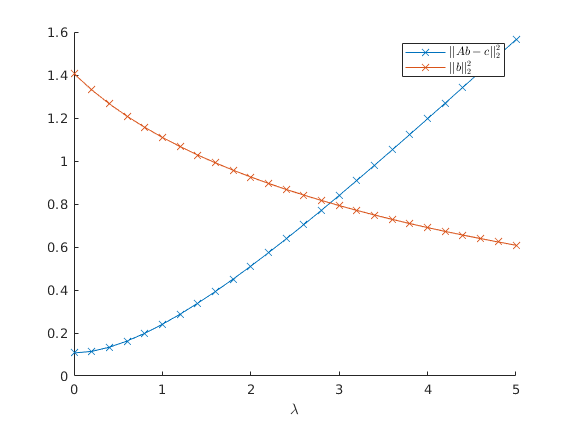
\includegraphics[width=\linewidth]{./1.png} \\
	\textit{Attachment: problem\_2\_b.m}
\end{sol}

\begin{problem}{3}
	Consider 3 people making dependent estimates of a number, with the following expectations of errors and correlations of errors:
	\begin{align*}
		E[\epsilon_1^2] &= 1773 \\
		E[\epsilon_2^2] &= 645 \\
		E[\epsilon_3^2] &= 1796 \\
		E[\epsilon_1\epsilon_2] &= 1057 \\
		E[\epsilon_1\epsilon_3] &= 970 \\
		E[\epsilon_2\epsilon_3] &= 708
	\end{align*}
	Compute the average of errors and the error of the average in this case.
\end{problem}
\begin{sol}
	The average of errors can be given by
	\begin{align*}
		E_{AE} &= \frac{1}{N} \sum_{i=1}^{N} E_x[\epsilon_i^2(x)] \\
			   &= \frac{1}{3} (1773+645+1796) \\
			   &= \frac{4214}{3}\\
	\text{The error of the average can} &\text{ be given by}\\
		E_{EA} &= \frac{1}{N^2} E_x[(\sum_{i=1}^{N}\epsilon_i(x))^2] \\
			   &= \frac{1}{9}(1773+645+1796+2\times 1057+2\times 970 + 2\times 708) \\
			   &= 1076
	\end{align*}
\end{sol}

\end{document}